\documentclass[14 pt]{extarticle}

	\usepackage[frenchb]{babel}
	\usepackage[utf8]{inputenc}  
	\usepackage[T1]{fontenc}
	\usepackage{amssymb}
	\usepackage[mathscr]{euscript}
	\usepackage{stmaryrd}
	\usepackage{amsmath}
	\usepackage{tikz}
	\usepackage[all,cmtip]{xy}
	\usepackage{amsthm}
	\usepackage{varioref}
	\usepackage{geometry}
	\geometry{a4paper}
	\usepackage{lmodern}
	\usepackage{hyperref}
	\usepackage{array}
	 \usepackage{fancyhdr}
	 \usepackage{float}
\renewcommand{\theenumi}{\alph{enumi})}
	\pagestyle{fancy}
	\theoremstyle{plain}
	\fancyfoot[C]{} 
	\fancyhead[L]{Feuille d'exercices}
	\fancyhead[R]{ novembre 2022}\geometry{
 a4paper,
 total={170mm,257mm},
 left=20mm,
 top=20mm,
 }
	
	
	\title{Exercices chapitre 3 - 2}
	\date{}
	\begin{document}

\begin{center}{\Large Exercices chapitre 3 - 2}\\ 
 \end{center}
 
 \section{Comparaison de fractions}
 
\subsection*{Exercice 1 : exercice-type}
On veut classer dans l'ordre croissant les fractions suivantes. 

\[ \frac12, \frac23, \ \frac34, \frac43, \frac 5{12}, \frac16, \frac76\]
\begin{enumerate}
\item Faire la liste des dénominateurs des fractions à classer. 
\item Quel est le plus petit nombre multiple de tous ces dénominateurs ? 
\item Réduire toutes les fractions précédentes à ce dénominateur. 
\item Classer les fractions dans l'ordre croissant. 
\item Où s'insérerait la fraction $\frac{8}{24}$ dans cette liste ?
\end{enumerate} 
 
 
 \subsection*{Exercice 2}
 
 Classez dans l'ordre croissant les fractions suivantes. 
 
 \[ \frac13,\ \frac7{5},\ \frac3{15},\ \frac29,\ \frac7{15},\ 
 \frac8{45}\]
 
 
 \subsection*{Exercice 3}
 
 Classez dans l'ordre décroissant les fractions suivantes. 
 
 \[ \frac1{12},\ \frac4{5},\ \frac8{15},\ \frac5{6},\ \frac7{30},\ 
 \frac3{4}\]
 
 \section{Repérage sur la demi-droite graduée}

 \subsection*{Exercice 4}
 
Sur la demi-droite graduée ci-dessous, placez une fraction sur chaque graduation visible.

\begin{figure}[H]
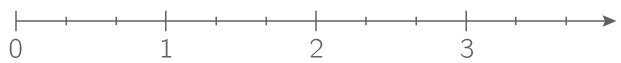
\includegraphics[width=15cm]{Axe.png}
\end{figure} 


\subsection*{Exercice 5}

Tracez une demi-droite graduée de 25 carreaux, et placez $5$ sur le $25^e$ carreau.
\begin{enumerate}
\item Exprimez la valeur d'une graduation sous la forme d'une fraction.
\item Pour chacun des nombres suivants, trouvez une fraction qui lui est égale et admet $5$ comme dénominateur : 
\[ \frac35; \ \ 
3; \ \ 
0,3; \ \ 
\frac{14}{10}; \ \ 
\frac{15}{25}; \ \ 
\frac{80}{25}; \ \ 
\frac{57}{15}; \ \ 
\frac{96}{20}\]

\end{enumerate}
 
 \subsection*{Exercice 6}
 
 Tracez une demi-droite graduée de 24 carreaux; et placez $1$ au troisième carreau. Placez-y les fractions suivantes : 
 
\[ \frac53; \ \ 
3; \ \ 
\frac{14}3; \ \ 
\frac{14}6; \ \ 
\frac{22}3; \ \ 
\frac{100}{15}; \ \ 
\frac{69}{9}; \ \ 
\frac{56}{14}\]
\section{Pourcentages}
\subsection*{Exercice 7 : des fractions aux pourcentages}

Exprimez les fractions suivantes comme des pourcentages. Si ce pourcentage s'écrit avec un nombre fini de chiffres après la virgule, écrivez-le en entier. Sinon, arrondissez au dixième le plus proche. 

\begin{enumerate}
\item $\frac14$,
\item $\frac1{25}$,
\item $\frac23$,
\item $\frac{4}{16}$,
\item $ \frac47$,
\item $\frac19$,
\item $\frac4{125}$,
\item $\frac1{64}$.
\end{enumerate}


\subsection*{Exercice 8 : des pourcentages aux fractions}

Exprimez les pourcentages suivants comme des fractions irréductibles.

\begin{enumerate}
\item $50\%$,
\item $1\%$,
\item $10\%$,
\item $25\%$,
\item $75\%$,
\item $12,5\%$,
\item $20\%$, 
\item $60\%$, 
\item $85\%$, 
\item $62,5\%$.
\end{enumerate}

 	\end{document}
